\documentclass[11pt, a4paper]{article}		% general format


%%%% Charset
\usepackage[utf8]{inputenc}					% use utf8					
\usepackage[russian]{babel}					% use russian font


%%%% Math
\usepackage{amsmath}						% Amer­i­can Math­e­mat­i­cal So­ci­ety (AMS) math fa­cil­i­ties
\usepackage{amsfonts}						% fonts from the AMS
\usepackage{amssymb}						% additional math symbols


%%%% Graphics
\usepackage{graphicx}


\author{Бусаров Владислав}
\title{Отчет по лабораторной работе №4 :\\ Утилита для исследования сети и сканер портов nmap}
\date{2015}

%---------------------------------------------------------

\begin{document}
\maketitle
\tableofcontents
\newpage

%---------------------------------------------------------


\section{Цель работы}

Определить набор и версии сервисов запущенных на компьютере в диапазоне адресов.
Данная работа выполняется на ОС Kali linux, используется утилита nmap.



%---------------------------------------------------------

\section{Ход работы}


%---------------------------------------------------------

\subsection{Провести поиск активных хостов}

Настройки сети: в нашей сети имеется всего 3 хоста.

\begin{itemize}
\item Windows 10 (192.168.0.104), основная ОС
\item kali linux (192.168.0.102)
\item metasploitable2 (192.168.0.105)
\end{itemize}

Выведем список хостов в подсети 192.168.0.0/24

Для этого воспользуемся командой \verb'nmap -sn 192.168.0.0/24'. (См. рисунок 1)

\begin{figure}[h!]
\centering
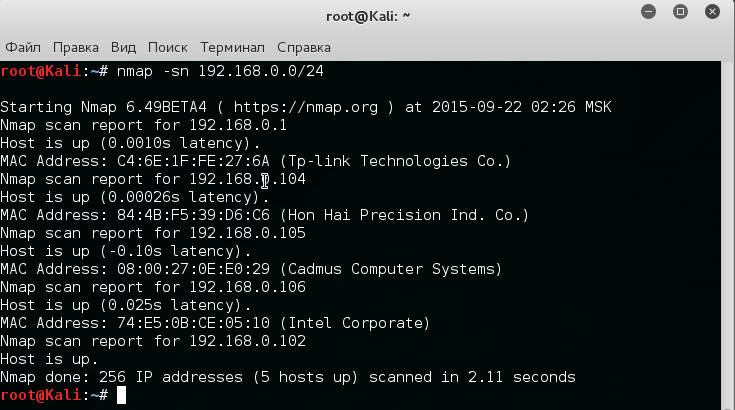
\includegraphics[scale=0.8]{res/1}
\caption{Поиск хостов}
\end{figure}

%---------------------------------------------------------

\subsection{Определить открытые порты}

Просканируем порты metasploitable2.

Для определения открытых портов достаточно просто ввести \verb'nmap 192.168.0.105' (сканируются порты до 1024). Или же воспользоваться опцией -p, например \verb'nmap -p "*" 192.168.0.105'. Данной командой просканируются все порты, если необходимо задать диапазон достаточно указать его вместо "*".
Результат на рисунке 2.

\begin{figure}[h!]
\centering
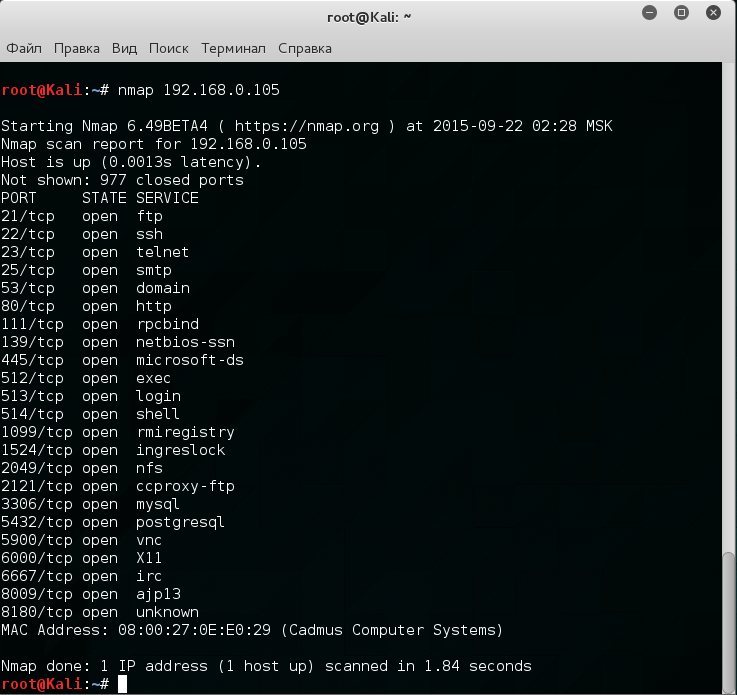
\includegraphics[scale=0.8]{res/2}
\caption{Поиск портов}
\end{figure}

%---------------------------------------------------------

\subsection{Определить версии сервисов}

Чтобы определить версии сервисов необходимо воспользоваться командой nmap с ключем sV следующим образом: \verb'nmap -sV 192.168.0.105'. 
Результат на рисунке 3.

\begin{figure}[h!]
\centering
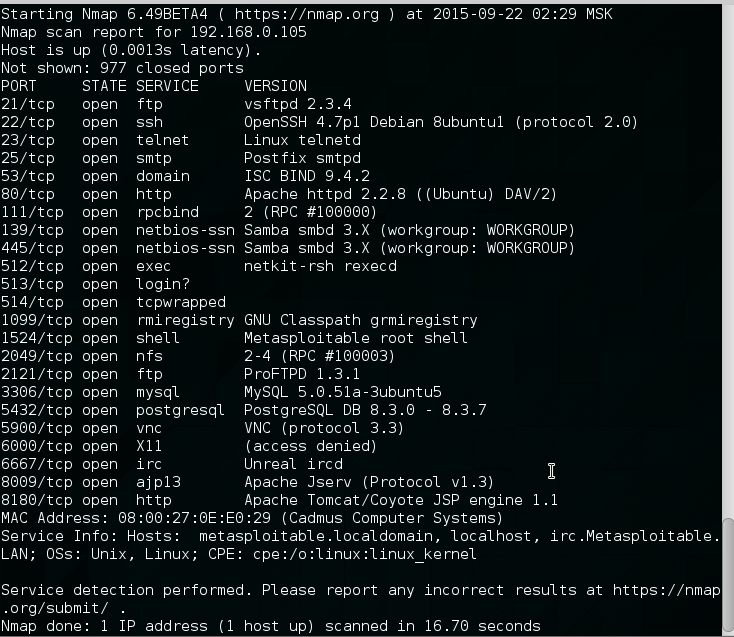
\includegraphics[scale=0.8]{res/3}
\caption{Определение версий сервисов}
\end{figure}

%---------------------------------------------------------

\subsection{Изучить файлы nmap-services, nmap-os-db, nmapservice-probes}

Рассмотрим файл nmap-services. Для этого введем команду 

vim /usr/share/nmap/nmap-services. 

Файл служит для быстрого поиска, напрмер с ключем -F. В файле в каждой строчке задаются сервисное название или сокращение, число порта и протокол, определенный разделом, частота порта мера того, как часто порт был найдет открытым во время сканирования. Пример файла можно увидеть на рисунке 4.


\begin{figure}[h!]
\centering
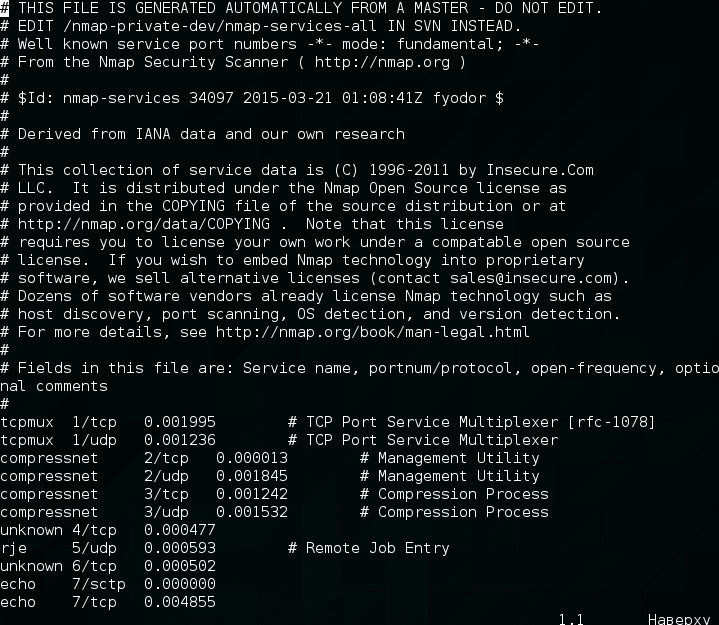
\includegraphics[scale=0.75]{res/4}
\caption{Файл nmap-services}
\end{figure}

Файл nmap-os-db содержит сотни примеров реакций ОС на nmap. Таким образом nmap определяет какая опреационная система установлена на удаленной машине. Для того чтобы узнать какая ОС установлена нужно запустить nmap с ключем -O. Содержимое файла представлено на рисунке 5.

\begin{figure}[h!]
\centering
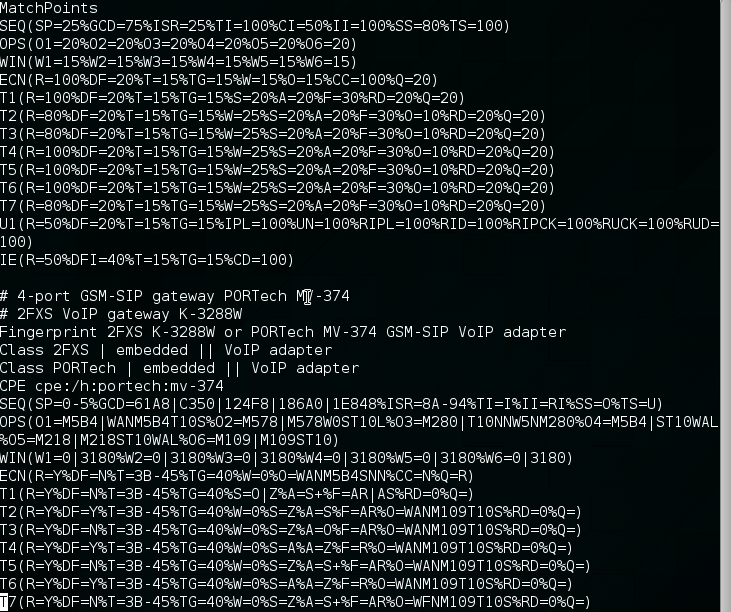
\includegraphics[scale=0.75]{res/5}
\caption{Файл nmap-os-db}
\end{figure}


nmap-service-probes — это простой текстовый файл состоящий из строк, в котором хнаняться тесты и сигнатуры подсистем определений версий. Строки, начинающиеся с символа "решетки" (\#) воспринимаются как комментарии и игнорируются обработчиком. Пустые строки также не обрабатываются. 


Синтаксис: 
\begin{itemize}
\item Probe <protocol> <probename> <probesendstring> - директива probe (тест) - указывает nmap, какие данные отправлять в процессе определения служб
\item match <service> <pattern> <productname> <version> <device> <h?????> <info> <OS> - указывает nmap на то, как точно определить службу, используя полученный ответ на запрос, отправленный предыдущей директивой probe. Эта директива используется в случае, когда полученный ответ полностью совпадает с шаблоном. При этом тестирование порта считается законченным, а при помощи дополнительных спецификаторов nmap строит отчет о названии приложения, номере версии и дополнительной информации, полученной в ходе проверки
\item softmatch <service> <pattern> <productname> <version> <device> <h?????> <info> <OS> - имеет аналогичный формат директиве match. Основное отличие заключается в том, что после совпадения принятого ответа с одним из шаблонов softmatch, тестирование будет продолжено с использованием только тех тестов, которые относятся к определенной шаблоном службе. Тестирование порта будет идти до тех пор, пока не будет найдено строгое соответствие (match) или не закончатся все тесты для данной службы
\item ports <portlist> - группирует порты, которые обычно закрепляются за идентифицируемой данным тестом службой
\item sslports <sslportlist> - аналогична директиве ports, только эта директива указывает порты, обычно используемые совместно с SSL
\item totalwaitms <milliseconds> - редко используемая, т.к. указывает сколько времени (в миллисекундах) необходимо ждать ответ, прежде чем прекратить тест службы
\end{itemize}

%---------------------------------------------------------

\subsection{Добавить новую сигнатуру службы в файл nmap-service-probes (для этого создать минимальный tcp server, добиться, чтобы при сканировании nmap указывал для него название и версию)}

Напишем простой tcp-сервер, который просто ждет подключения клиента и отправляет ему сообщение. В файл nmap-service-probes добавим следующую строку: 

\verb"match tcp-server m|^111| v/1.0.X/ p/Busarov V.A./ i/LoL It's works heh/"

Код сервера:

\begin{verbatim}
using System;
using System.Collections.Generic;
using System.Linq;
using System.Text;
using System.IO;
using System.Net;
using System.Net.Sockets;
using System.Threading;

namespace ExampleTcpListener_Console
{
    class ExampleTcpListener
    {
        static void Main(string[] args)
        {
            TcpListener server = null;
            try
            {
                int MaxThreadsCount = Environment.ProcessorCount * 4;
                Console.WriteLine(MaxThreadsCount.ToString());
                ThreadPool.SetMaxThreads(MaxThreadsCount, MaxThreadsCount);
                ThreadPool.SetMinThreads(2, 2);

                Int32 port = 9596;
                IPAddress localAddr = IPAddress.Parse("192.168.0.104");
                int counter = 0;
                server = new TcpListener(localAddr, port);

                server.Start();

                while (true)
                {

                    Console.Write("\nWaiting for a connection... ");

                    ThreadPool.QueueUserWorkItem(ObrabotkaZaprosa, server.AcceptTcpClient());
                    counter++;
                    Console.Write("\nConnection №" + counter.ToString() + "!");

                }
            }
            catch (SocketException e)
            {
                Console.WriteLine("SocketException: {0}", e);
            }
            finally
            {
                server.Stop();
            }

            Console.WriteLine("\nHit enter to continue...");
            Console.Read();
        }

        static void ObrabotkaZaprosa(object client_obj)
        {
            Byte[] bytes = new Byte[256];
            String data = null;

            TcpClient client = client_obj as TcpClient;

            data = null;

            NetworkStream stream = client.GetStream();

            int i;

            data = "111";
            byte[] msg = System.Text.Encoding.ASCII.GetBytes(data);
            stream.Write(msg, 0, msg.Length);

            client.Close();
        }
    }
}
\end{verbatim}
  
Таким образом теперь nmap знает, что если при пустом запросе с сервера прихоит строка 111, значит нужно выводить информацию которая указана на рисунке 6.

\begin{figure}[h!]
\centering
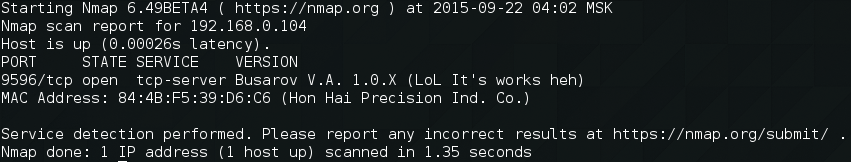
\includegraphics[scale=0.8]{res/6}
\caption{Вывод информации о сервисе}
\end{figure}



%---------------------------------------------------------

\subsection{Сохранить выводы утилиты в формате xml}

Для того, чтобы вывести данные в xml файл достаточно вызвать команду nmap с ключем -oX и указать имя файла. Например: 

\verb'nmap -sn -oX output.xml 192.168.0.104'

Результат можно увидеть на рисунке 7:

\begin{figure}[h!]
\centering
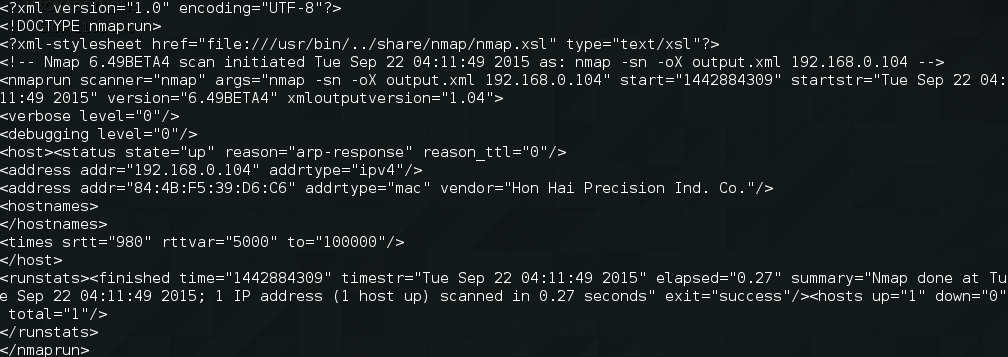
\includegraphics[scale=0.8]{res/7}
\caption{output.xml}
\end{figure}

%---------------------------------------------------------

\subsection{Исследовать различные этапы и режимы работы nmap с использованием утилиты Wireshark}

Wireshark — это достаточно известный инструмент для захвата и анализа сетевого трафика.
Wireshark работает с подавляющим большинством известных протоколов, имеет понятный и логичный графический интерфейс на основе GTK+ и мощнейшую систему фильтров.
Кроссплатформенный, работает в таких ОС как Linux, Solaris, FreeBSD, NetBSD, OpenBSD, Mac OS X, и, естественно, Windows. Распространяется под лицензией GNU GPL v2. Доступен бесплатно на сайте wireshark.org.

Далее продемонстрируем простую работу с wireshark. 
Будем сканировать порты используя ключ -xS (xmas tree). В данном режиме отправляются tcp пакеты с установленными флагами FIN, URG, PASS.
В случае если порт закрыт придет пакет с флагом RST (прерывание соединения), иначе нисего не должно прийти. Приступим.
При запуске wireshark предложит выбрать интерфейс и начать сканировать его траффик(см. рисунок 8). Выберем интерфейс eth0

\begin{figure}[h!]
\centering
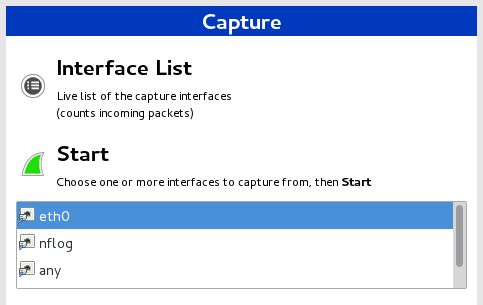
\includegraphics[scale=0.8]{res/wireshark_int}
\caption{wireshark выбор интерфейса и старт}
\end{figure}

Wireshark по-умолчанию выводит все пакеты, которые проходят через интерфейс eth0. Все пакеты просматривать неудобно, поэтому мы будем пользоваться фильтрами. Поставим фильтр по протоколу tcp.

Введем команду сканирования порта 21 на ОС metasploitable2: 

\verb'nmap 192.168.0.105 -p21 -sX'

Результат на рисунке 9. Увидим два пакета, ответа на которые не пришло, значит порт открыт.

\begin{figure}[h!]
\centering
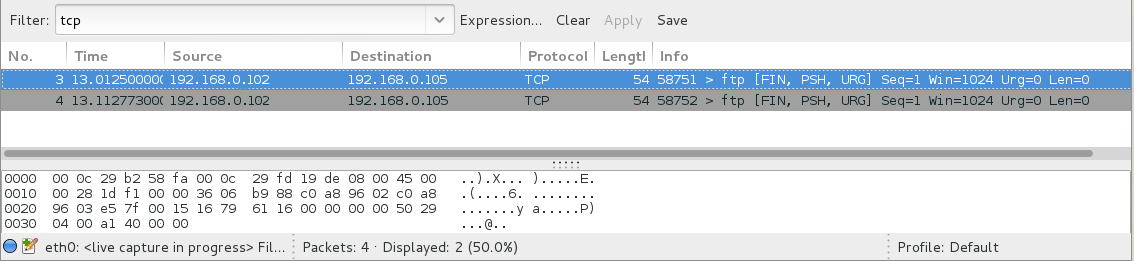
\includegraphics[scale=0.8]{res/xmas_scan_21}
\caption{xmas scan порт 21}
\end{figure}

Введем команду сканирования порта 43 на ОС metasploitable2: 

\verb'nmap 192.168.0.105 -p43 -sX'

Результат на рисунке 10. Увидим два пакета, первый - наш запрос, второй - ответ с флагом RST. Значит порт закрыт.

\begin{figure}[h!]
\centering
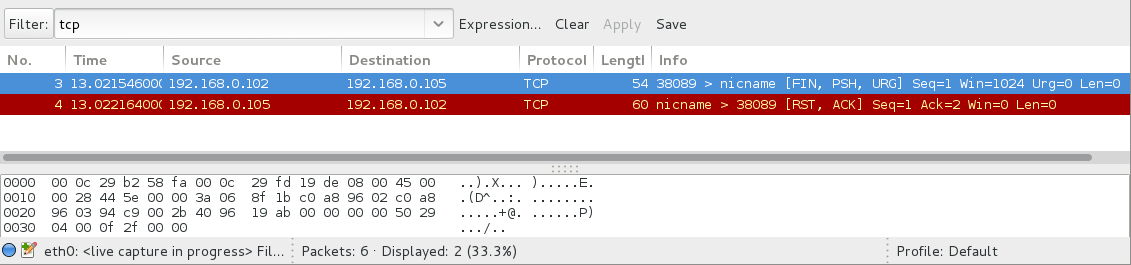
\includegraphics[scale=0.8]{res/xmas_scan_43}
\caption{xmas scan порт 43}
\end{figure}

Так же было проведено сканирование по всем портам, результаты совпадают с SYN сканированием и connect(). В отличие от сканирования основной ОС (Windows 10). В которой на закрытые порты не отправлялся ответ с флагом RST. Результаты на рисунке 11. Windows не придерживаются стандарта RFC 793. Так же не по стандарту работают системы Cisco, BSDI, HP/UX, MVS, IRIX. Они передают пакет RST при сканировании открытых портов.

\begin{figure}[h!]
\centering
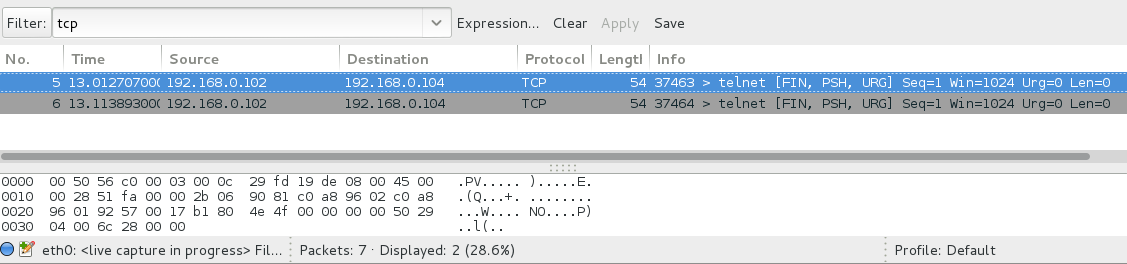
\includegraphics[scale=0.8]{res/xmas_scan_23}
\caption{xmas scan порт 23 (Windows 10)}
\end{figure}


%---------------------------------------------------------

\subsection{Просканировать виртуальную машину Metasploitable2 используя nmap\_db из состава metasploit-framework}

Для работы с metasploit потребуется СУБД postgresql. Для того, чтобы ее запустить воспользуемся командой 

\verb'service postgressql start'

Затем запустим msf консоль командой \verb'msfconsole'.

В данной консоли осуществляется работа с metasplit. Проверим соединение с БД:

\verb'db_status'

Результат на рисунке 13.

\begin{figure}[h!]
\centering
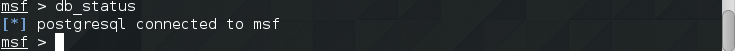
\includegraphics[scale=0.8]{res/8}
\caption{db\_status}
\end{figure}

Таблицы БД: hosts, services, vulns, loot и notes. В каждой храниться соответствующая информация.
Для заполнения этих таблиц автоматизированно, можно использовать db\_nmap. Так же можно использовать какую-то любую утилиту для сканирования, экспортировать результаты её работы в XML-файл, а потом - импортировать его в метасплойт. Это можно сделать, использовав db\_import внутри меню метасплойт.

Выполним команду: \verb'db_nmap -sV 192.168.0.0/24'

Вывод будет такой же как и при использовании команы nmap. Теперь после того как была просканирована наша сеть можно посмотреть, что было записано в БД: \verb'hosts', \verb'services'. Результаты на рисунках 13 и 14.

\begin{figure}[h!]
\centering
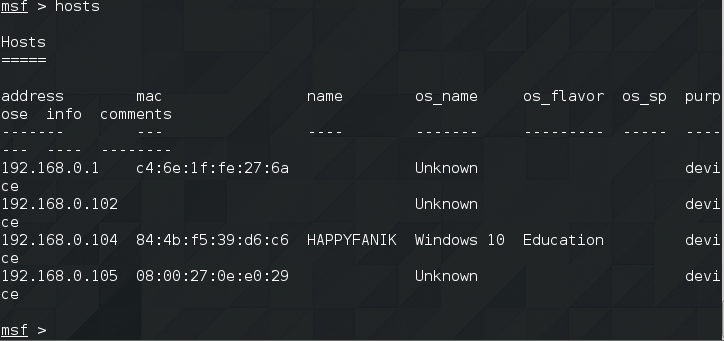
\includegraphics[scale=0.8]{res/9}
\caption{Таблица хостов}
\end{figure}

\begin{figure}[h!]
\centering
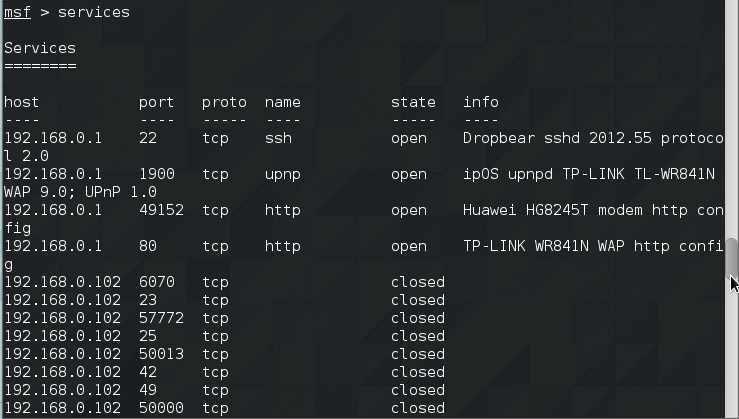
\includegraphics[scale=0.8]{res/10}
\caption{Таблица сервисов}
\end{figure}

%---------------------------------------------------------

\subsection{Выбрать пять записей из файла nmap-service-probes и описать их работу. Выбрать один скрипт из состава Nmap и описать его работу}

\begin{itemize}
\item Первая запись

Возьмем самую первую запсись probe - эта запись теста с отправкой null-запроса. В данной записи будет отправляться пустой запрос по протоколу TCP. С ожиданием ответа в 6 секунд(директива totalwaitms).

\begin{figure}[h!]
\centering
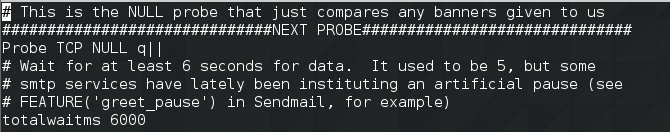
\includegraphics[scale=0.8]{res/11}
\caption{Запись 1}
\end{figure}

\item Вторая запись

Второй записью рассмотрим match после probe null-запроса. Если пользователь укажет ключ -sV при использовании nmap и после отправки нулевого теста с сервера приедет выражение подходящее под mSxf5xc6x1a тогда в колонке SERVICE при выводе информации он увидит наименование сервиса 1c-server, а в олонке VERSION 1C:Enterprise business management server.

\begin{figure}[h!]
\centering
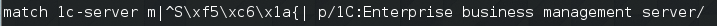
\includegraphics[scale=0.8]{res/12}
\caption{Запись 2}
\end{figure}

\item Третья запись

В данной запись на сервер отправляется запрос по протоколу TCP в котором передается информация. Так же указан список портов и ssl-портов, по которым нужно осуществлять сканирование.

\begin{figure}[h!]
\centering
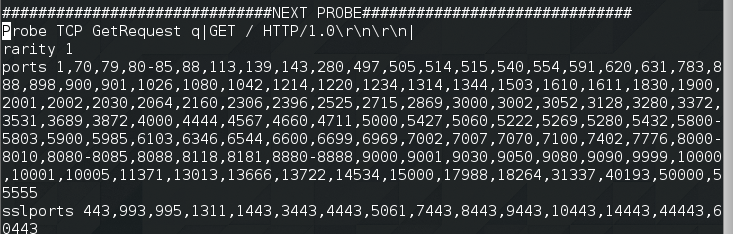
\includegraphics[scale=0.8]{res/13}
\caption{Запись 3}
\end{figure}

\item Четвертая запись

Здесь отправляется запрос по протоколу UDP для проверки RPC.

\begin{figure}[h!]
\centering
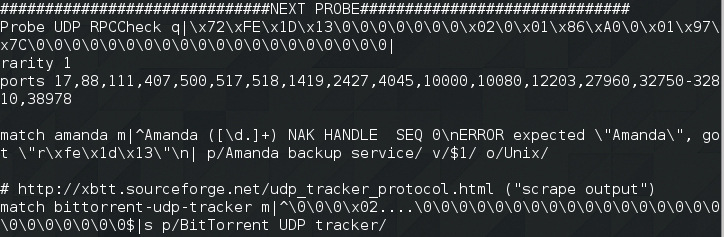
\includegraphics[scale=0.8]{res/14}
\caption{Запись 4}
\end{figure}

\item Пятая запись

Здесь отправляется запрос по протоколу UDP для проверки sql, через порт 1434.


\begin{figure}[h!]
\centering
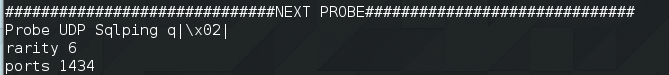
\includegraphics[scale=0.8]{res/15}
\caption{Запись 5}
\end{figure}




\item Скрипт

Рассмотрим следующий скрипт \verb'skypev2-version.nse'. Его можно найти в папке с отчетом.

Первым делом в нем объявлены переменные импортированные из библиотек:

\begin{verbatim}
local comm = require "comm"
local nmap = require "nmap"
local shortport = require "shortport"
local string = require "string"
local U = require "lpeg-utility"
\end{verbatim}

Далее следует описание скрипта в переменной \verb'description':

\begin{verbatim}
description = [[
Detects the Skype version 2 service.
]]
\end{verbatim}

Далее описание в комментарии в формате NSEDoc.

\begin{verbatim}
---
-- @output
-- PORT   STATE SERVICE VERSION
-- 80/tcp open  skype2  Skype
\end{verbatim}

Далее имя автора, лицензия, категория:

\begin{verbatim}
author = "Brandon Enright"
license = "Same as Nmap--See http://nmap.org/book/man-legal.html"
categories = {"version"}
\end{verbatim}

Далее правило порта(вместо него можно задавать правило хоста) - функция возвращающая true или false. Если возвращает true, то выполняется функция заданная в перемнной action. В данном случае из кода понятно, в каких случая выполняется это условие.
 
\begin{verbatim}
portrule = function(host, port)
  return (port.number == 80 or port.number == 443 or
    port.service == nil or port.service == "" or
    port.service == "unknown") -- условия по портам
  and port.protocol == "tcp" and port.state == "open" -- условия по протоколу
  and port.version.name_confidence < 10 -- доверие
  and not(shortport.port_is_excluded(port.number,port.protocol)) -- порт не исключен
  and nmap.version_intensity() >= 7 -- версия интенсивности
end
\end{verbatim}

Далее приведен код функции action:

\begin{verbatim}
action = function(host, port)
  local result, rand
  -- Did the service engine already do the hard work?
  if port.version and port.version.service_fp then
    -- Probes sent, replies received, but no match.
    result = U.get_response(port.version.service_fp, "GetRequest")
    -- Loop through the ASCII probes most likely to receive random response
    -- from Skype. Others will also recieve this response, but are harder to
    -- distinguish from an echo service.
    for _, p in ipairs({"HTTPOptions", "RTSPRequest"}) do
      rand = U.get_response(port.version.service_fp, p)
      if rand then
        break
      end
    end
  end
  local status
  if not result then
    -- Have to send the probe ourselves.
    status, result = comm.exchange(host, port,
      "GET / HTTP/1.0\r\n\r\n", {bytes=26})

    if (not status) then
      return nil
    end
  end

  if (result ~= "HTTP/1.0 404 Not Found\r\n\r\n") then
    return
  end

  -- So far so good, now see if we get random data for another request
  if not rand then
    status, rand = comm.exchange(host, port,
      "random data\r\n\r\n", {bytes=15})

    if (not status) then
      return
    end
  end

  if string.match(rand, "[^%s!-~].*[^%s!-~].*[^%s!-~]") then
    -- Detected
    port.version.name = "skype2"
    port.version.product = "Skype"
    nmap.set_port_version(host, port)
    return
  end
  return
end
\end{verbatim}

После прохождения всех проверок, обозначается версия и продукт(после комментария Detected).

Для использования скрипта нужно ввести либо ключ -sC, либо --script=<имя\_скрипта>.

Для примера была просканирована основная ОС. Двумя способами. Результаты можно увидеть на рисунках 20 и 21.

\begin{figure}[h!]
\centering
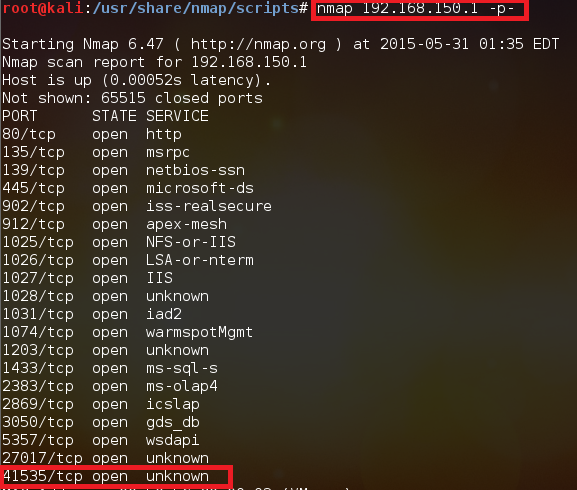
\includegraphics[scale=0.8]{res/script_1}
\caption{Результаты сканирования без использования скрипта}
\end{figure}

\begin{figure}[h!]
\centering
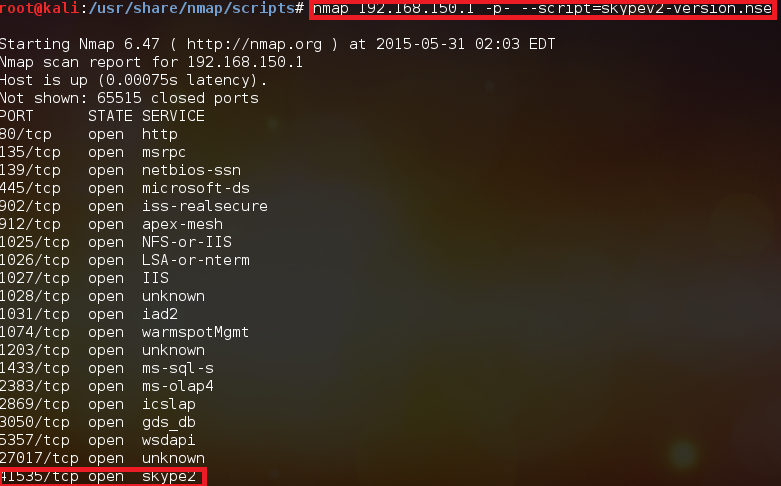
\includegraphics[scale=0.8]{res/script_2}
\caption{Результаты сканирования с использованием скрипта}
\end{figure}

\end{itemize}

%---------------------------------------------------------

\section{Вывод}

В ходе проделанной работы были изучены основы работы с nmap, немного изучен сниффер wireshark, а так же запись в БД metasploit посредством команды db\_nmap. Ранее я не был знаком с подобными программами, поэтому не с чем сравнивать. В общем интересно было посканировать хосты и порты. Понравилось сканировать трафик через wireshark. Так же понравилось писать свой сервер для порта. 


\end{document}